\section{Preliminary Experiments}\label{preliminary-experiments}

\{\#sec:experiment\}

\begin{quote}
\emph{We have some idea as to the intricate design of the puppet and the
puppet strings, but we lack insight into the mind of the puppeteer.}

--- Bizzi \& Ajemian, \emph{2020}
\end{quote}

\subsection{Goals}\label{goals}

\begin{itemize}
\tightlist
\item
  measure across learning
\item
  analyze this learning sequence to find traces of what's being learned
  at a trajectory level
\item
  gain inspiration for what might be modeled
\end{itemize}

\subsection{Recording Setup}\label{recording-setup}

The concept of the experimental setup is shown in \{+@fig:setup\}, where
32 monopolar electrodes are attached to a subject's forearm to record
muscle activity. The arm and hand are kinematically constrained in a
custom fixture and motor activity is recorded during low-level isometric
muscle contractions. The setup circumvents the limb biomechanics by
mapping muscle output directly to virtual stimuli shown on a screen. By
focusing on low-force, isometric contractions we intend to avoid
complications due to artifacts in dynamic, high-force movements.

\begin{figure}
\phantomsection\label{fig:setup}
\centering
\includegraphics[width=1\textwidth,height=\textheight]{images/hardware/setup.pdf}
\caption{(a) Graphic depicting the closed-loop EMG interface concept in
a center-hold, reach-out type task. The multidimensional EMG signal is
transformed online through a mapping \(F\) from EMG electrode space to a
lower dimensional task space. In experiments shown here the task space
is a two-dimensional, though the EMG interface can be extended to tasks
with higher-dimensional inputs. The subject's arm and hand are
constrained during the experiment to ensure isometric contractions. (b)
First prototype of custom recording hardware consisting of four bands of
eight electrodes each, and a spherical hand constraint. Our recordings
are 32 channel monopolar recording with reference electrode at the
wrist. (c) Example cup-style monopolar recording electrodes, 5mm in
diameter. (d) Side view of the recording hardware. Also pictured is the
arm restraint frame to ensure isometric contractions. The frame obscures
the subject's arm from view and contains adjustable elbow and wrist
rests. (d) Recording hardware shown off the arm with wireless amplifier
and connection board.}\label{fig:setup}
\end{figure}

As far as we are aware, this setup is novel in combining a high number
of channels with an abstract mapping. Learning experiments have used
joint angles and a few muscles (typically movements of the wrist or
pairs of thumb and intrinsic hand muscles), but none have taken a
data-driven approach in constructing a virtual learning environment in
the style of cortical
BMI{[}@BergerDifferencesInAdaptationRates2013a;@Dyson2018;@radhakrishnanLearningNovelMyoelectricControlled2008;@Gallego2017{]}.
Our EMG recording setup is custom-built: the ``Sessantaquattro'' EMG
amplifier was acquired from OT Bioelettronica, the electronic connector
was designed in-house, the electrodes were acquired from Medkit UK, and
the recording software was written in a mixture of Bonsai (C\#) and
Python. EMG is acquired at 2kHz sample rate with 24-bit precision. A
clip of raw data is shown in \{+@fig:raw\_data\}.

\begin{figure}
\phantomsection\label{fig:raw_data}
\centering
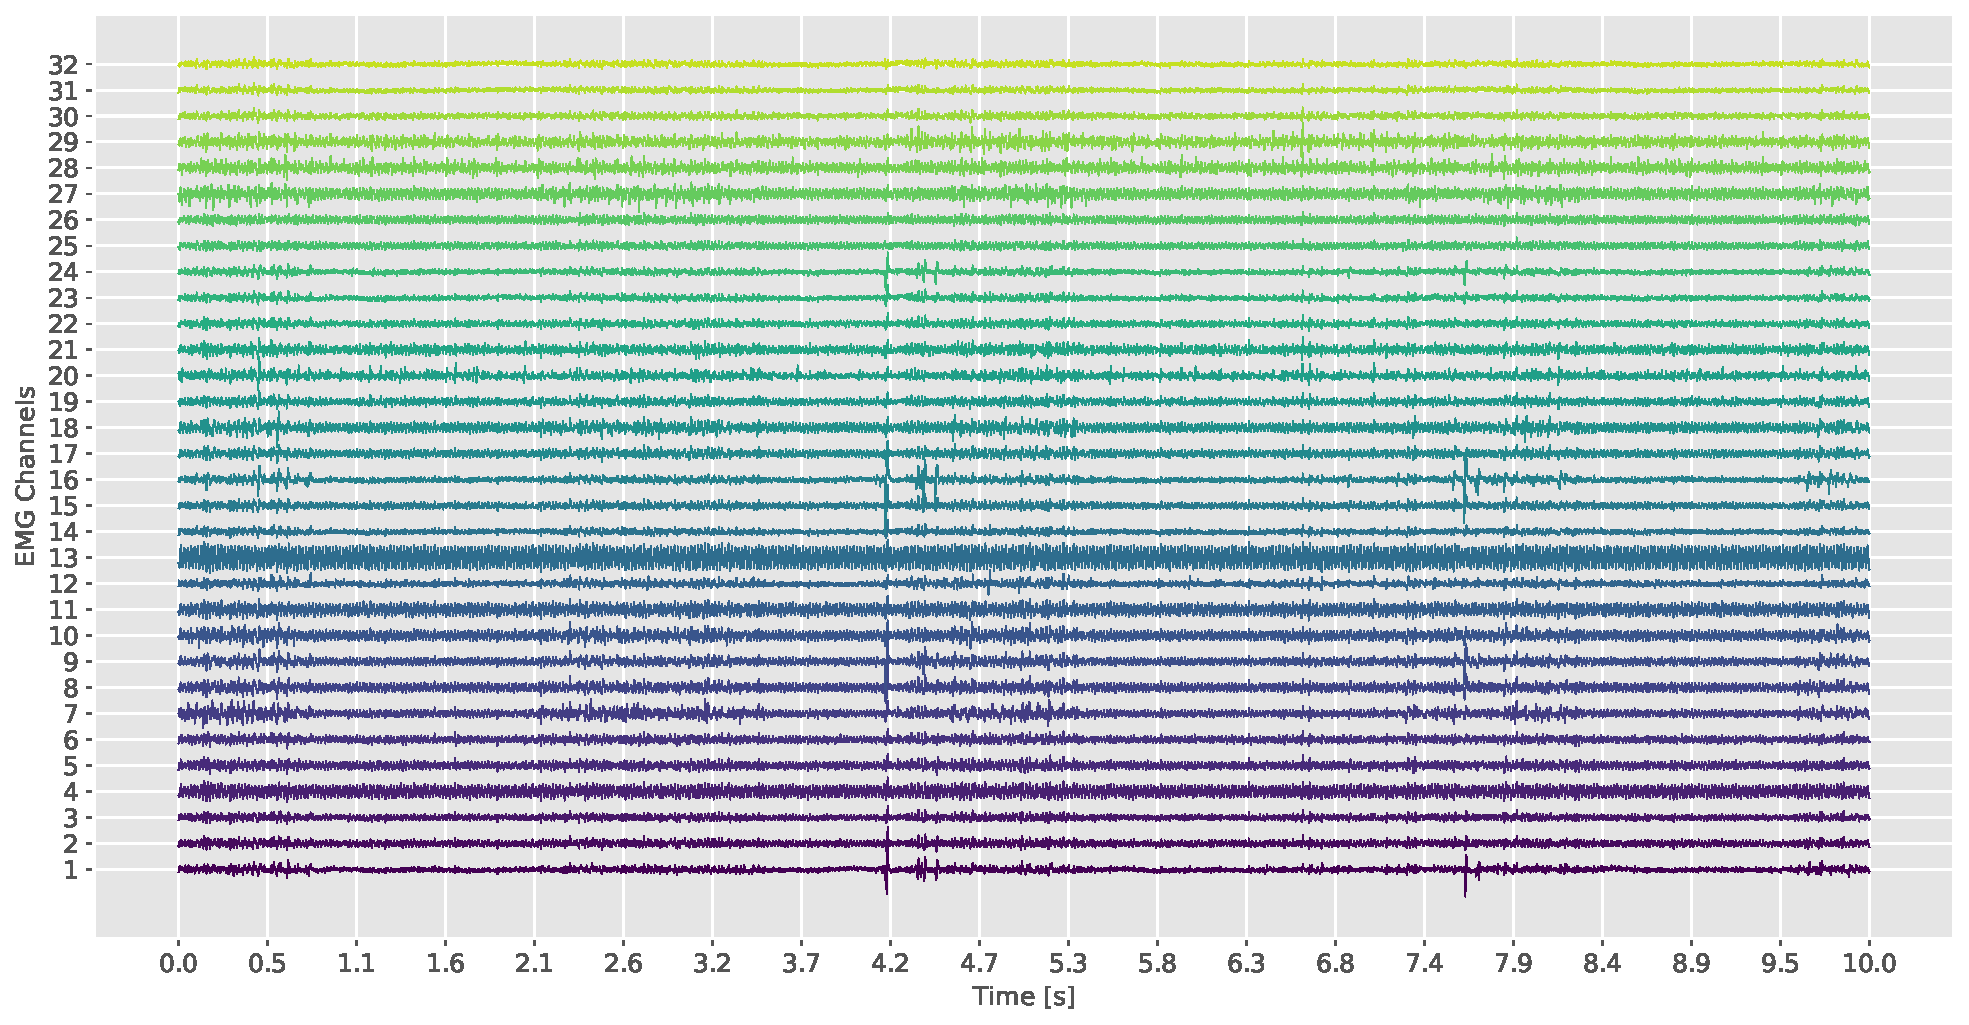
\includegraphics[width=1\textwidth,height=\textheight]{images/data_analysis/fingers/raw_data.pdf}
\caption{10 seconds of raw 32-channel EMG data taken during a minimal
finger flexion trial. Note that some channels include a nontrivial
amount of line noise. This noise will be drastically reduced through
changes being made in the next recording hardware revision which include
shielding, shorter cables, and better cable routing. Note that some
channels (e.g.~channel 24) show very low noise and putative single motor
unit action potentials can be seen on many
channels.}\label{fig:raw_data}
\end{figure}

To preprocessing the data, simple filtering and rectifying were applied,
as is commonly done in the
literature{[}@sangerBayesianFilteringMyoelectric2007;@churchlandNeuralPopulationDynamics2012a;@churchlandNeuralVariabilityPremotor2006;@sussillo2015{]}.
As shown in \{+@fig:preprocessing\_steps\}, here we apply highpass
filtering at 40Hz to remove any low-frequency oscillations and DC
offsets, rectification and lowpass filtering at 5Hz to extract what is
typically associated with a force readout of the EMG signal in the case
that electrodes are positioned over the belly of a single muscle. These
filter parameters were chosen by visual comparison across a range of
values. While these preprocessing steps are in accordance with the
literature and yield a signal with frequencies on a behavioral timescale
though, as discussed in \{+@sec:next\_steps\}, preprocessing of raw EMG
signals is an area worth investigating the development and application
of more advanced methods.

\begin{figure}
\phantomsection\label{fig:preprocessing_steps}
\centering
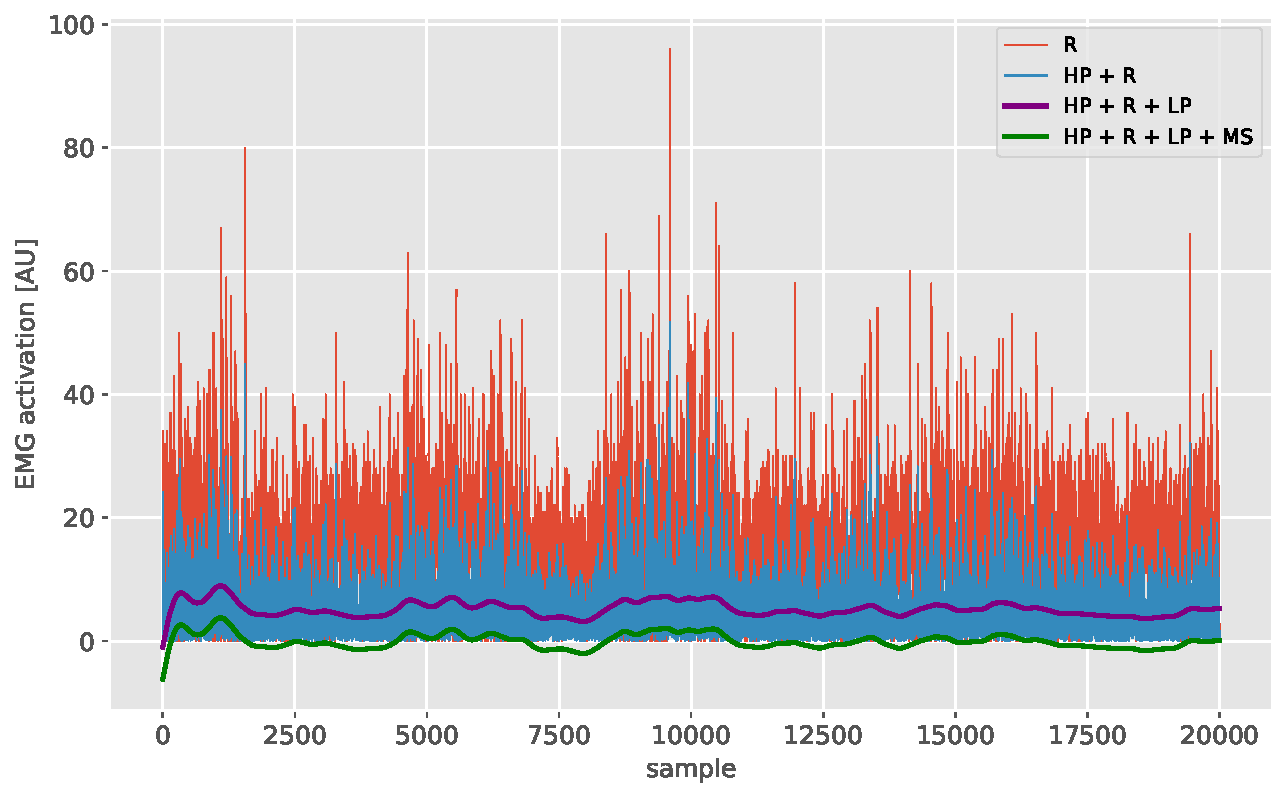
\includegraphics[width=1\textwidth,height=\textheight]{images/data_analysis/fingers/preprocessing_steps.pdf}
\caption{Data from a single trial showing each step of preprocessing.
The prototype preprocessing pipeline is highpass at 50Hz, rectification,
and lowpass at 5Hz. The within-trial, per-channel means are subtracted
from each trial. This matches what is typically done in the literature
to find a correlate of intended
force{[}@sangerBayesianFilteringMyoelectric2007;@churchlandNeuralPopulationDynamics2012a;@churchlandNeuralVariabilityPremotor2006;@sussillo2015{]}.
There is significant room for improvement on this workflow, as discussed
in the text.}\label{fig:preprocessing_steps}
\end{figure}

\subsection{Open-loop Finger
Recordings}\label{open-loop-finger-recordings}

In our first preliminary experiment, a single subject produced flexions
and extensions of each finger in the recording setup without any kind of
artificial feedback. One trial was collected per finger movement in
three blocks per session and one session per day over five days for a
total of fifteen trials per finger movement. The purpose of this
experiment is to determine the robustness over trials and sessions of
EMG features for a simple low-contraction movement, as well as to
determine the level of noise and artifacts in the data. Such baseline
measurements are important to properly decompose variability due to
electrode placement and exogenous noise from behavioral and
physiological variability in order to ensure reproducibility of our
results. Additionally, this baseline task may prove useful as a
benchmark for later tasks in terms of testing analysis and decomposition
techniques. A plot of all 32 channels for a single trial after
preprocessing is shown in \{+@fig:preprocessed\_data\}.

\begin{figure}
\phantomsection\label{fig:preprocessed_data}
\centering
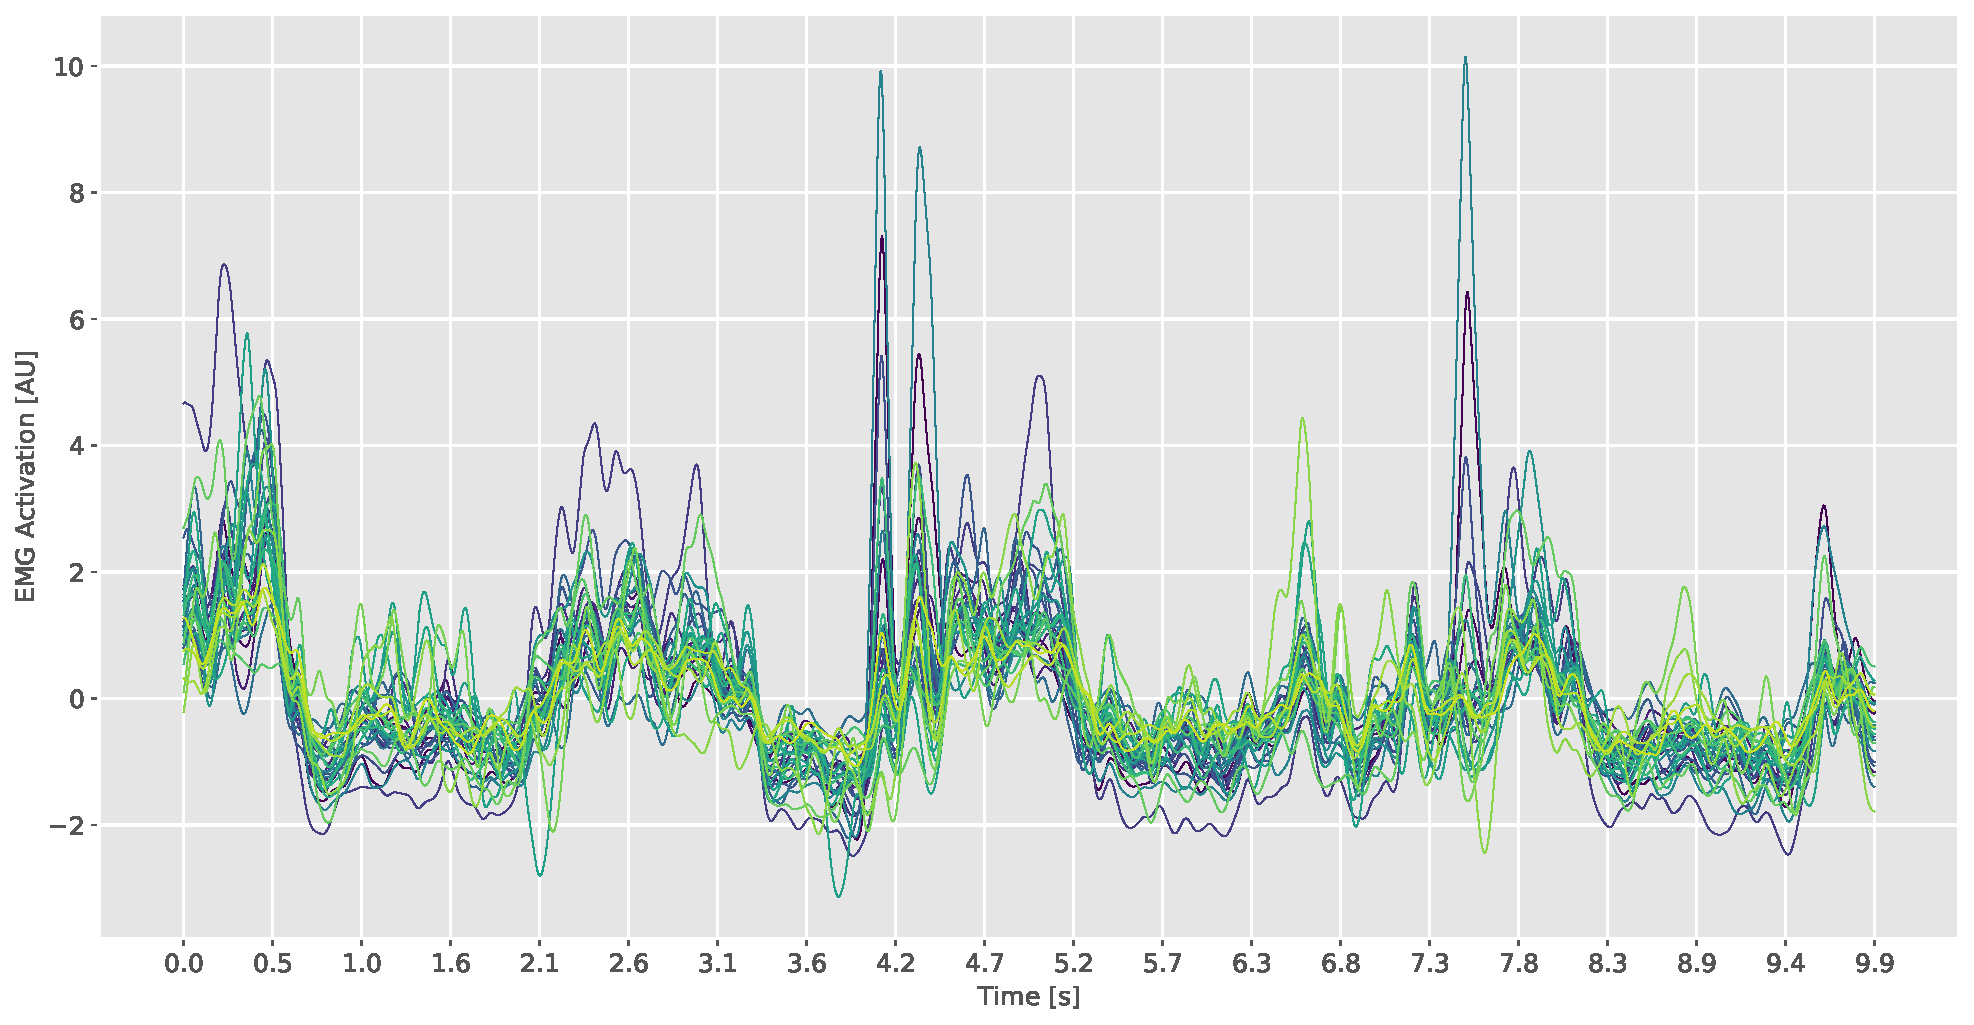
\includegraphics[width=1\textwidth,height=\textheight]{images/data_analysis/fingers/preprocessed_data.pdf}
\caption{All channels of data from a single trial after preprocessing.
Note the difference in baseline for each channel. Ideally, each channel
has a clear baseline of no activity, as further discussed in the main
text.}\label{fig:preprocessed_data}
\end{figure}

We first asked whether PCA applied to each individual trial would
extract a single, high-variance component reflecting the dimensionality
of the behavior. Since each finger movement is intuitively one
dimensional, we predict that PCA would find a single high-variance
component when run on each individual trial. As shown in
\{+@fig:PCA\_variances\}, this is generally the case, though there are
some outlier trials. After inspecting these outlier trials, it is likely
that the subject moved multiple fingers in these trials counter to the
experimenter's instruction.

\begin{figure}
\phantomsection\label{fig:PCA_variances}
\centering
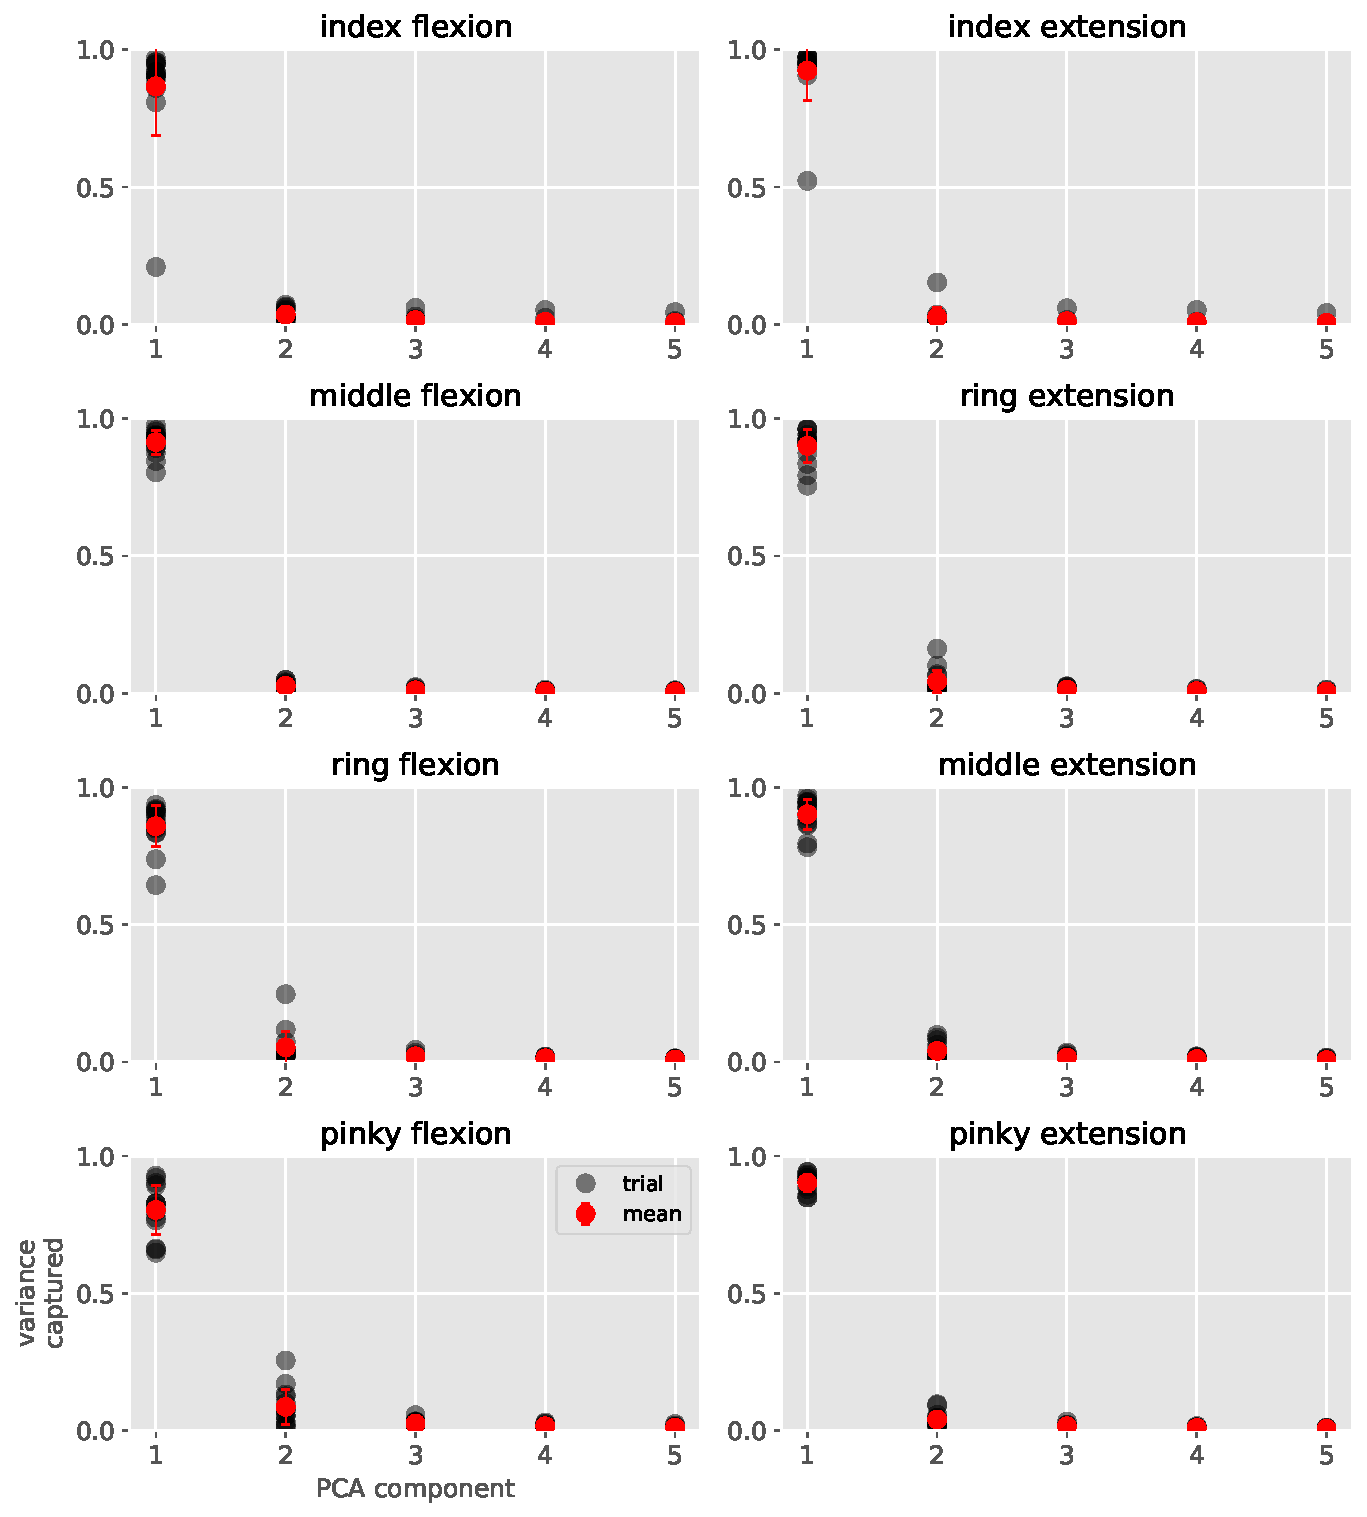
\includegraphics[width=1\textwidth,height=\textheight]{images/data_analysis/fingers/PCA_variances.pdf}
\caption{Fraction of variance captured by the top 5 principle components
for trials of single finger extensions and flexions. PCs were computed
for individual trials. Trials were recorded from one subject for 10s
each trial with finger movement frequency approximately 1Hz. Three
blocks each with one trial per finger movement were recorded per day for
5 days for a total of 15 trials per finger. Electrodes were not removed
between blocks but were removed between days. Each trial displays a
single high-variance PC component.}\label{fig:PCA_variances}
\end{figure}

We next asked, since each trial appeared to be dominated by a single
principle component, whether this top component was stable across trials
and across days. If the top component is stable, it implies that the
recording apparatus is robust to electrode movement between sessions.
The top components for each movement after running PCA on each trial are
shown in \{+@fig:PCA\_components\}. While it is not typical to run PCA
on individual trials, for the purpose of visually inspecting the PCA
weights over EMG channels it is used here.

\begin{figure}
\phantomsection\label{fig:PCA_components}
\centering
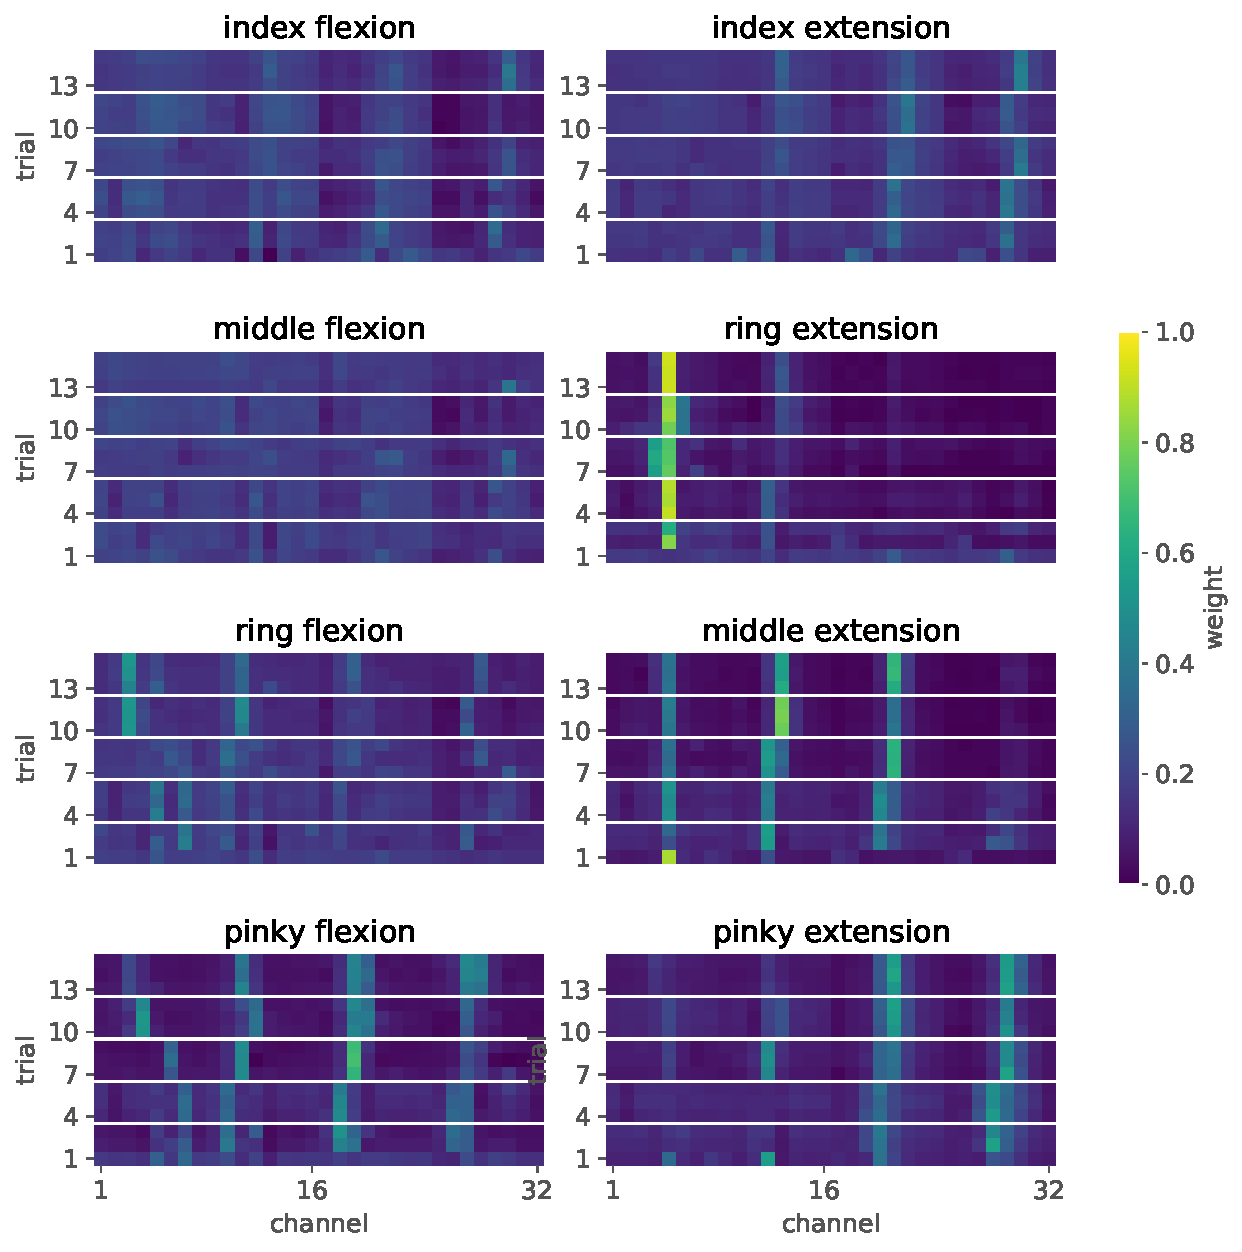
\includegraphics[width=1\textwidth,height=\textheight]{images/data_analysis/fingers/PCA_components.pdf}
\caption{The top principle component from each single finger movement
trials plotted as weights across channels. PCA was computed for each
trial individually. White horizontal lines show breaks between days when
electrodes were removed and reapplied. Each trial's top component is
relatively stable across trials and across days, though there is drift
and dropout of weights. Measures to increase cross-session stability are
discussed in the main text. Movements appear to vary between strong
localization on single channels and broad activation across
channels.}\label{fig:PCA_components}
\end{figure}

The results here suggest that, at least up to linear decompositions, the
features of low-contraction movements is relatively robust across
sessions. As discussed in \{+@sec:next\_steps\}, we will construct more
reliable means to place electrodes on subjects' forearms to further
increase repeatability. Another aspect of these results is our
assumption subjects are producing the same contraction each time they
move their finger, and at the same contraction level. That is, we assume
they are recruiting the same motor units each movement. This may not be
the case, and constructing new analyses which infer motor unit
activations may be useful to mitigate this issue.

\subsection{Center-hold Reach-out
Task}\label{center-hold-reach-out-task}

In this task, the 32-dimensional EMG electrode activity vector is mapped
to a 2D force acting on a point mass shown on the screen. The mapping
\(M\in\mathbb{R}^{2x32}\) maps 8 ``columns'' each consisting of 4
electrodes placed in a line down the length of the forearm each to one
of 2D root of unity. Each column of electrodes is thus mapped to one of
8 two-dimensional force vectors. In this experiment, the point mass has
zero inertia and zero friction and as such displays a direct, though
redundant, readout of the EMG signal. The task asks the subject to reach
one of 32 equally spaced targets on each trial. Subjects must hold in
the center of the task space for a designated period of time, after
which the target appears. Subjects then have a time window reach the
target. Data from one subject was recorded for three blocks in one
session. Each block consisted of 32 trials, one per target in a
randomized order.

The mapping between EMG and task space \(M\) can be written as

\[
M = \begin{bmatrix}\tilde{M} & \tilde{M} & \tilde{M} & \tilde{M}\end{bmatrix}
\]

where \(\tilde{M}\) consists of 8 equally spaced directions, one for
each ``column'' of the 4 EMG electrode bands around the subject's arm:

\[
\tilde{M} =
\begin{bmatrix}
0  & 0.71  & 1   & 0.71   & 0  & -0.71  & -1  & -0.71 \\
1  & 0.71  & 0  & -0.71  & 1   & -0.71   & 0   & 0.71
\end{bmatrix}
\]

A graphic showing the mappings from electrodes to force directions is
shown in \{+@fig:columns\}. While there are 8 possible force vectors the
subject can modulate by controlling the electrode activity on each of
her 8 columns, the EMG mapping is ultimately a projection onto the 2D
plane. Since the EMG signal is nonnegative, the subject could
technically modulate just four modes of electrode activity, the minimum
number needed to span the task space, to reach all 32 targets. This
mapping was chosen in order to provide a simple starting point to
explore the virtual EMG task. There are no added environmental dynamics,
only a redundant readout of force, and the signal is processed online in
the same manner as in the offline analyses. This task or a variant we
think can serve as a foundation upon which we can build more complex
mappings and virtual environments. Task space trajectories from each
block are shown in \{+@fig:trajectories\}. The fraction of trials
resulting in hold timeouts, reach timeouts, and target hits are shown
over blocks in \{+@fig:hit\_fraction\}.

\begin{figure}
\phantomsection\label{fig:columns}
\centering
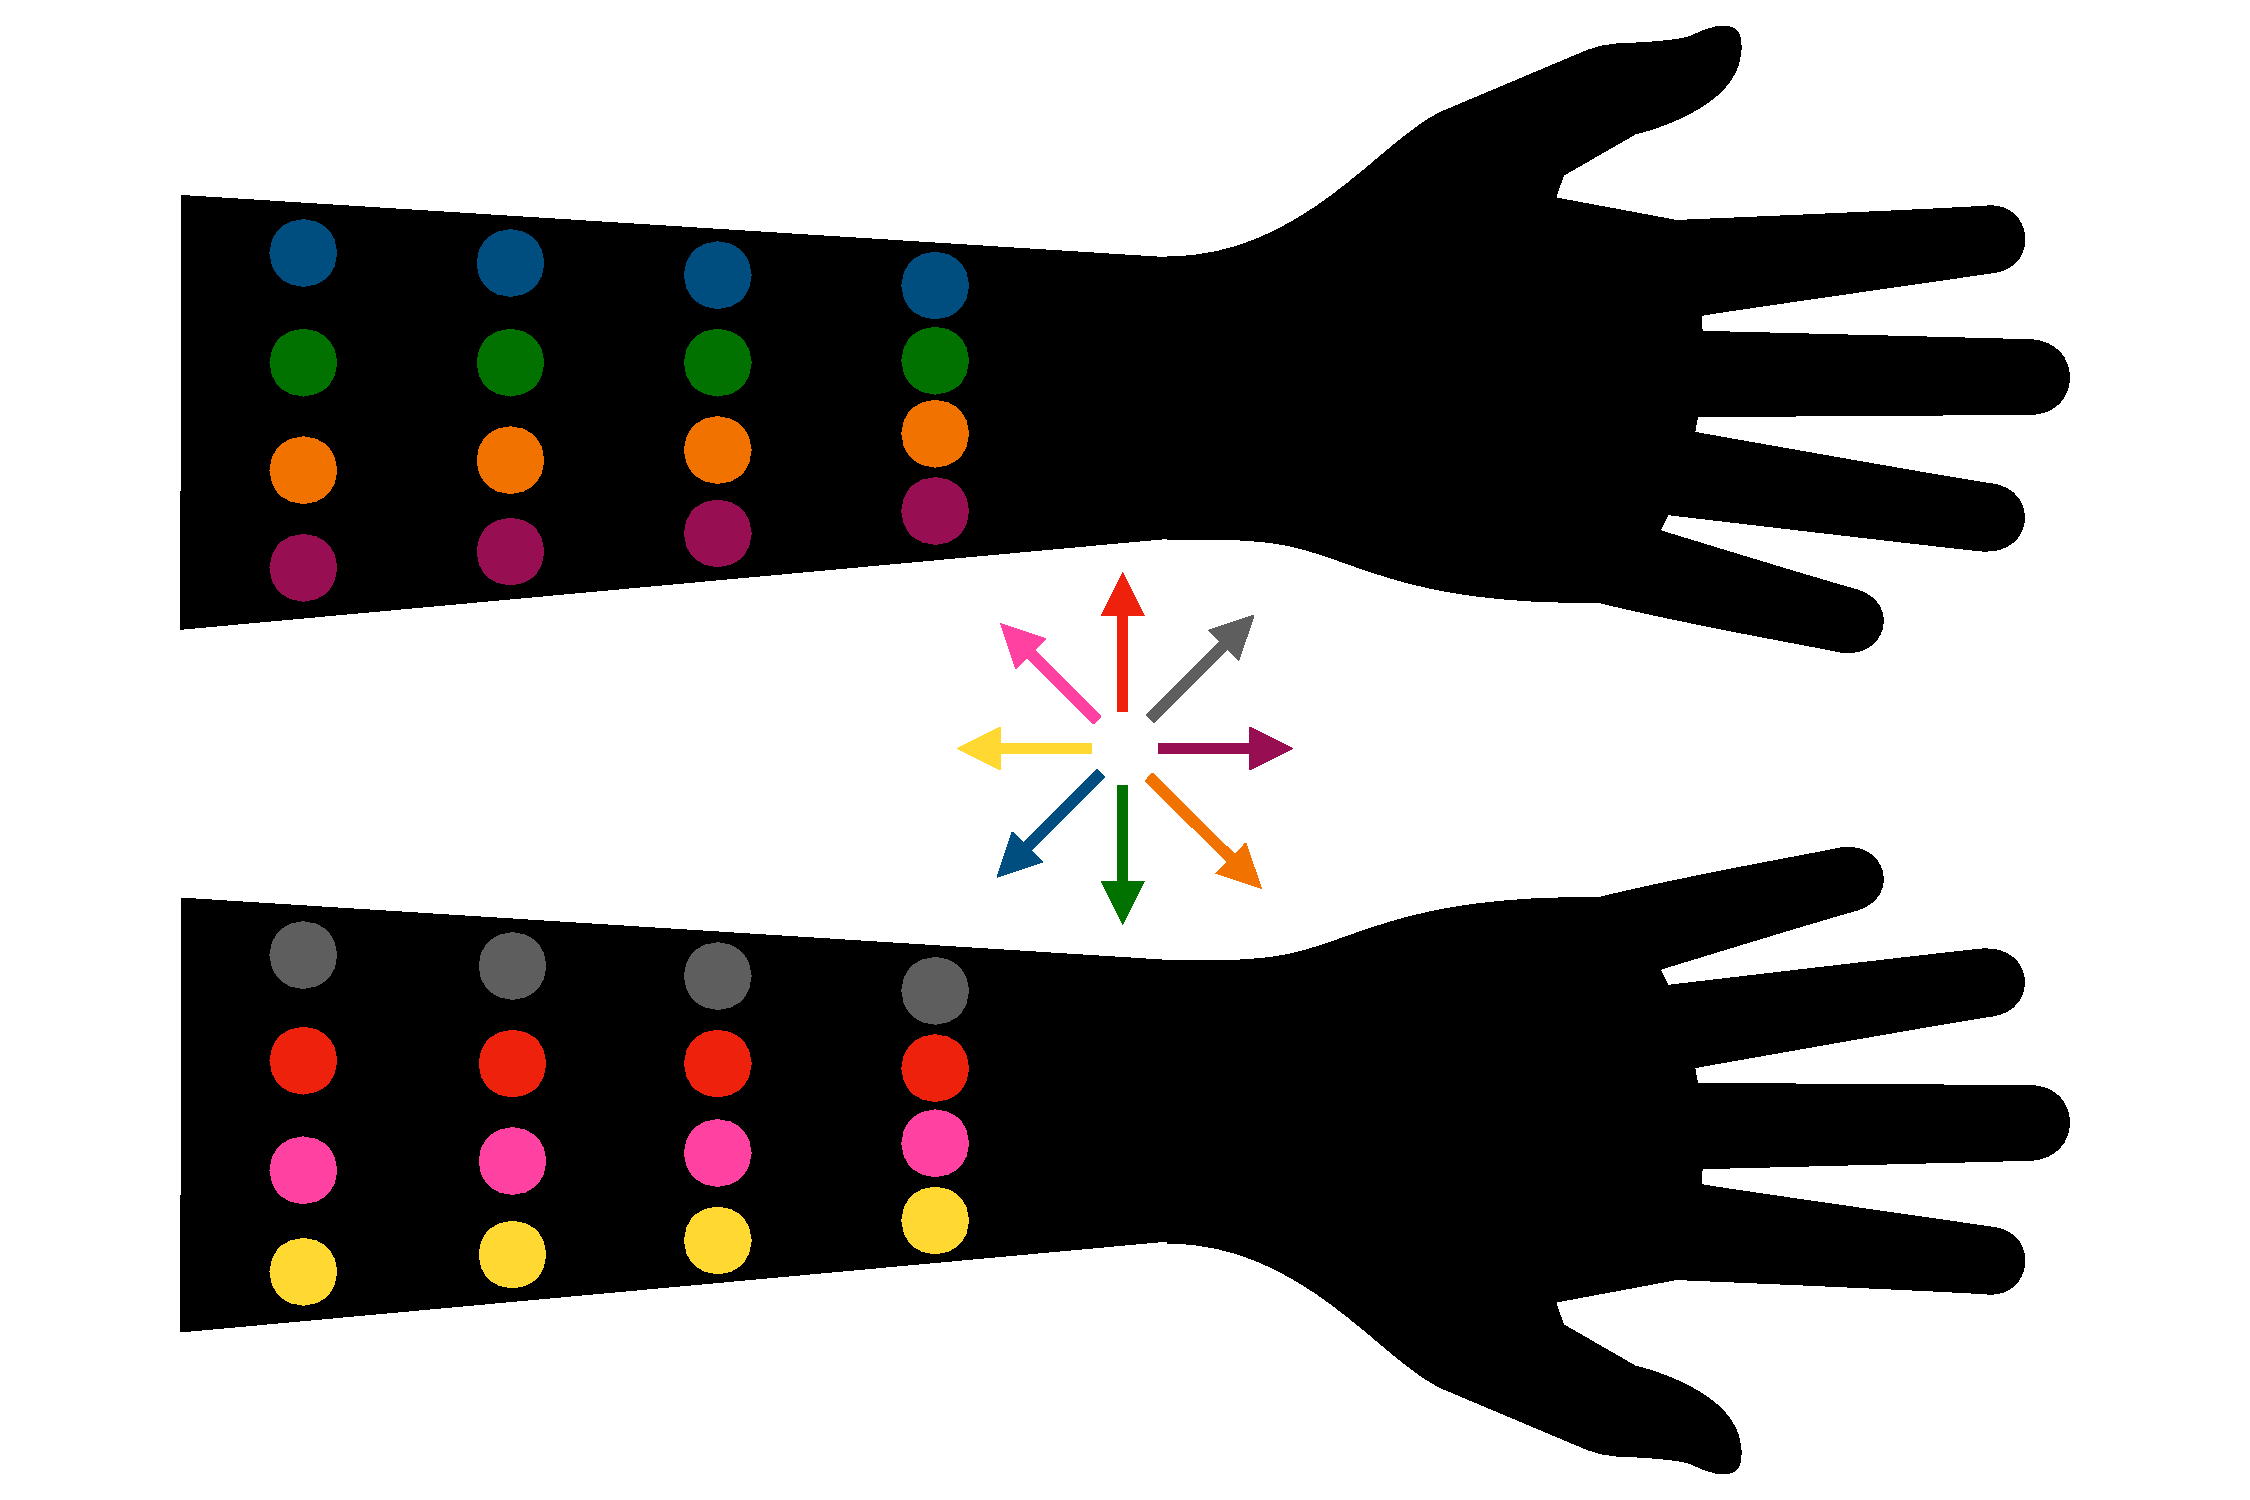
\includegraphics[width=0.7\textwidth,height=\textheight]{images/hardware/columns.pdf}
\caption{Graphic showing the mapping between electrodes in the
32-channel center-hold reach-out experiment to eight 2D force directions
in the virtual task space. Each of the eight columns consists of four
electrodes each mapped to the same force direction (denoted with
matching color) acting on a virtual point particle.}\label{fig:columns}
\end{figure}

\begin{figure}
\phantomsection\label{fig:trajectories}
\centering
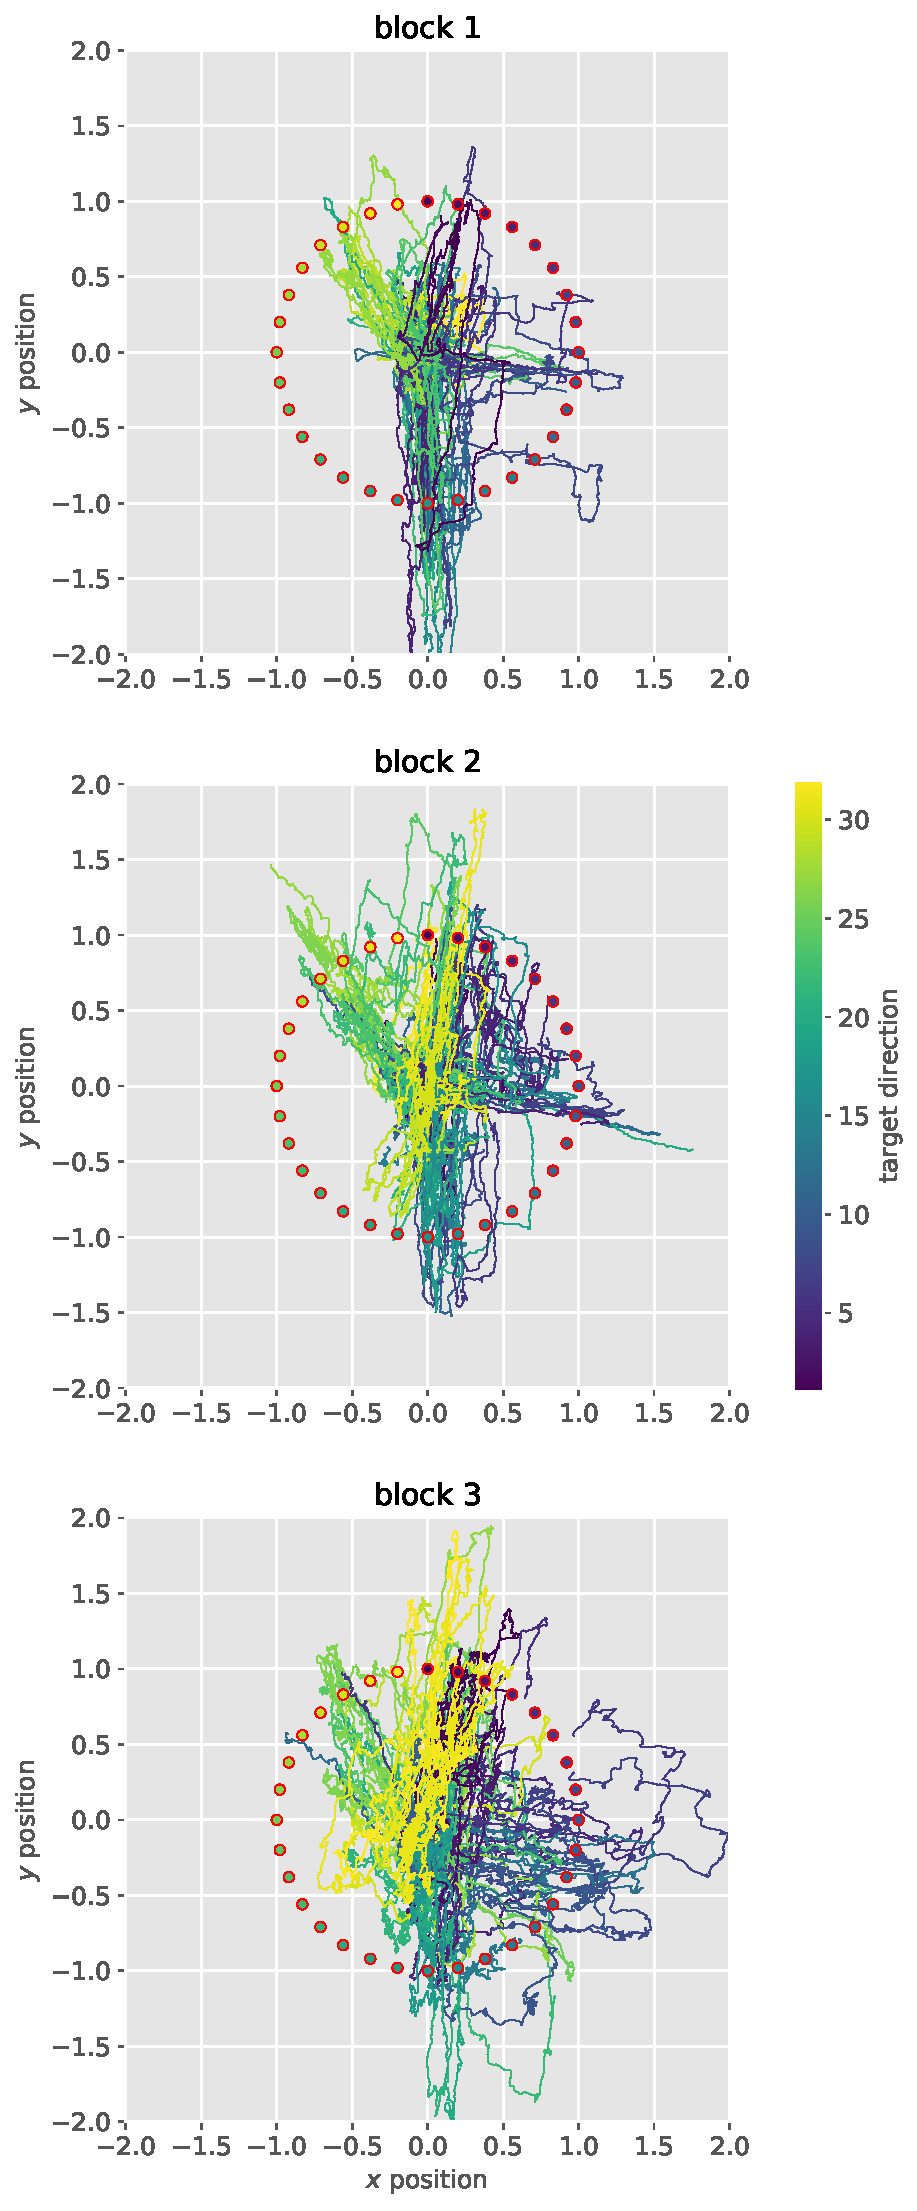
\includegraphics[width=0.6\textwidth,height=\textheight]{images/data_analysis/center_hold/trajectories.pdf}
\caption{Point mass position trajectories in two-dimensional task space
during the center-hold, reach-out task with 32 targets spaced evenly
around the unit circle (shown with red borders). Color corresponds to
target numbers, with target zero located at (0,1). Target order was
randomized. Training was conducted over 3 blocks each with 32 trials, 1
trial per target.}\label{fig:trajectories}
\end{figure}

\begin{figure}
\phantomsection\label{fig:hit_fraction}
\centering
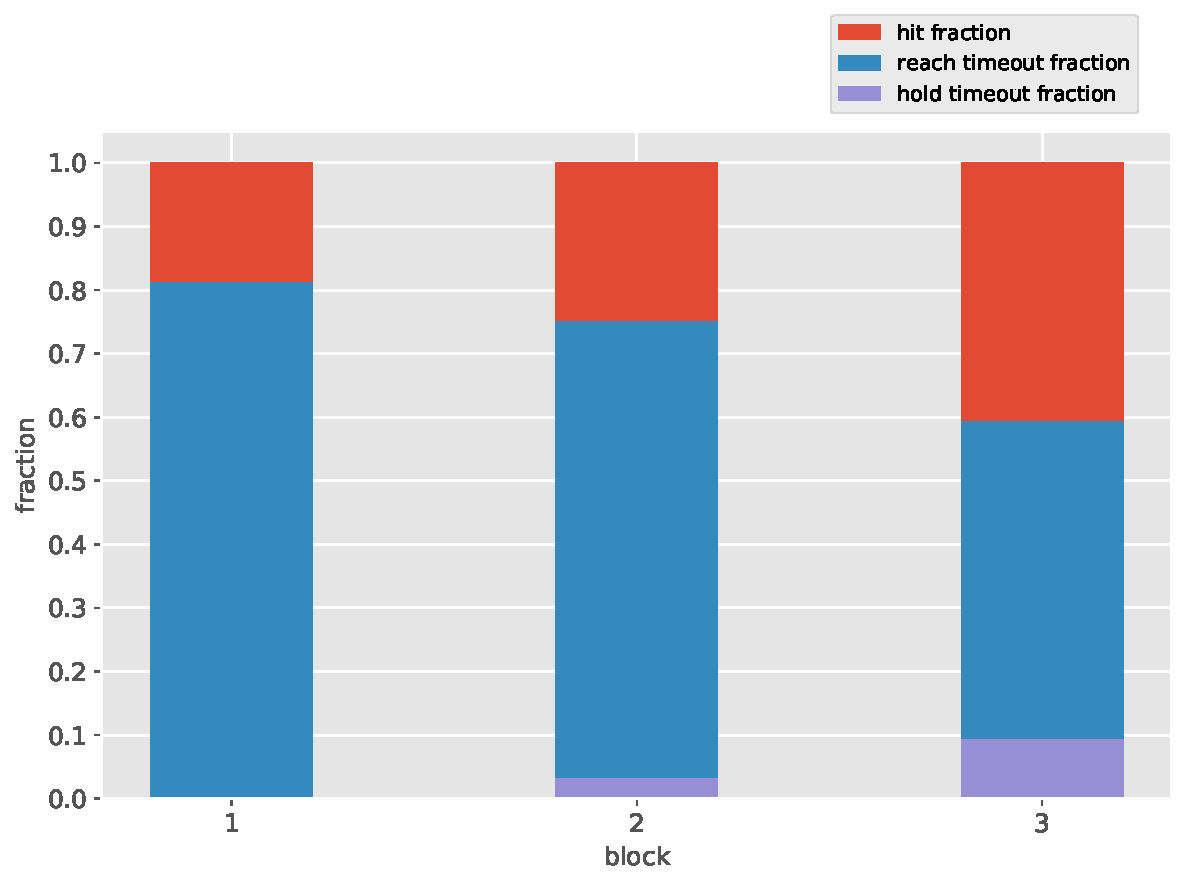
\includegraphics[width=0.7\textwidth,height=\textheight]{images/data_analysis/center_hold/hit_fraction.pdf}
\caption{Fractions of trial outcome types for each block of the
center-hold, reach-out task. Hit fraction increases on each trial,
suggesting the beginnings of task learning. Hold timeout failure
increases over trials as well, perhaps suggesting increased baseline
excitation of muscles during the hold period. Part of learning to
activate certain muscle modes is learning to inhibit
others.}\label{fig:hit_fraction}
\end{figure}

In this task, the subject's first goal is to interact through the
mapping \(M\) and learn the consequences of various motor activations.
That is, they must internalize a model of the virtual environment, what
might be called a system identification problem. Subjects must collect
data containing motor outputs and their sensory consequences. To do
this, they must explore the space of activity. We predict that over
trials, subjects' EMG activities over channels will become more varied
as they attempt new movement patterns to achieve their twin goals of
learning to move in this new environment and reaching the target.
Running PCA on each individual trial's EMG time series, we hypothesize
that initially we will see multiple components share signal variance as
subjects explore. Eventually, we would expect to see a decrease in this
measure of movement complexity a subjects hone their reaching skill.
Trial-level PCA component variance fractions are shown in
\{+@fig:PCA\_trial\_variance\}. We find an initial decrease in the top
component's variance fraction, though we expect many more trials will be
needed to see skill acquisition in the form of a dominant movement mode
per trial.

\begin{figure}
\phantomsection\label{fig:PCA_trial_variance}
\centering
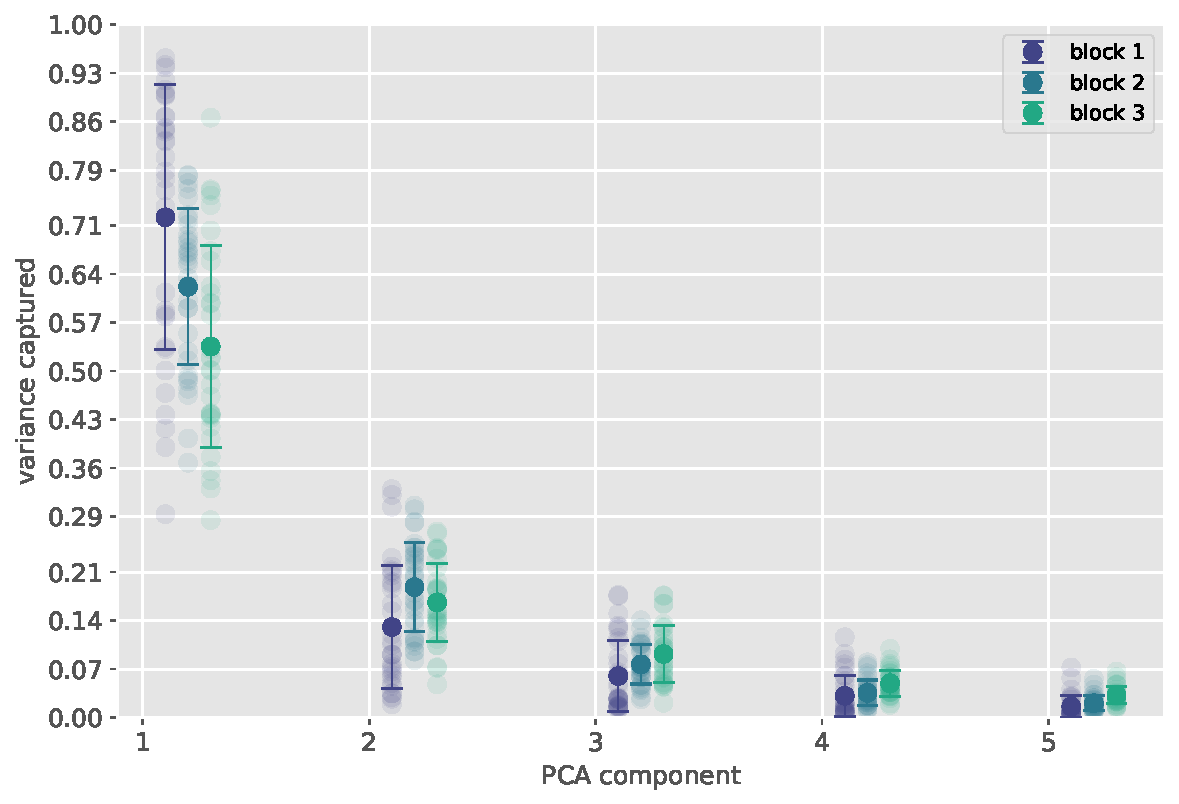
\includegraphics[width=0.7\textwidth,height=\textheight]{images/data_analysis/center_hold/PCA_trial_variance.pdf}
\caption{Fraction of variance captured by the top five principle
components when PCA is run on the EMG time series' of individual trials
of the center-hold, reach-out task. Error bars are standard deviation.
Over blocks, we see a slight decrease in the mean of the top component's
variance fraction, though with high variance. This may suggest greater
exploration within-trial, as less variance is captured by a single
component over blocks, though it could reflect more varied dynamics
across trials as the subject discovers new, task-relevant
activations.}\label{fig:PCA_trial_variance}
\end{figure}

We might model this task as the subject selecting an EMG signal \(x\)
which minimizes the distance between a target position \(b\) and the
projection of the EMG signal through the mapping \(M\) as well as
minimizes the norm of \(x\) in order to conserve metabolic energy. This
optimization can be written as a regularized least squares problem:

\[
\min_x\frac{1}{2}||Mx - b||^2_2 + \frac{\lambda}{2}||x||_2^2.
\]

This problem is known to have a unique minimum for \(\lambda>0\) which
is an approximation \(Mx\approx b\) regardless of the shape or rank of
\(M\). This implies that the subject, if they are biophysically capable
to do so, will learn distinct motor outputs for each target rather than
reusing modes for multiple targets with different activation levels.
That is the subject will, over time, learn to fractionate their muscle
output to reach their goal in order to minimize effort. For instance, to
reach the the target at position \((1,0)\) in Cartesian coordinates, the
subject could activate a bespoke activity mode and activate a
combination of two or more modes for targets at \(\pm45^\circ\) from
this central target. If this is the case, the model predicts that the
dimensionality of the EMG signal will increase over the course of
training as the subject learns to construct bespoke activity modes for
each target.

In \{+@fig:PCA\_concat\_variance\} we compute PCA on the concatenation
of all trials within blocks for which we predict an increase in the
number of dominant EMG modes as subjects learn multiple movements to
reach individual targets. We expect subjects to, over time, develop some
number of bespoke movement modes to activate independently and as a
composition to reach each target. We find a suggestion of this idea in
the data with our basic PCA analysis. More trials, session, and subjects
will be required to explore this idea, and we are investigating
probabilistic measures of signal complexity such as entropy to formalize
this hypothesis. One direction might be to further define this task a
regularized regression with different regularization terms chosen
normatively for different sections of the learning and control process,
and fitting data to these predictions. For instance, early in training
subjects may not optimize for target accuracy as much as for signal
sparsity, whereas later in learning subjects may optimize for target
accuracy and output signal magnitude.

\begin{figure}
\phantomsection\label{fig:PCA_concat_variance}
\centering
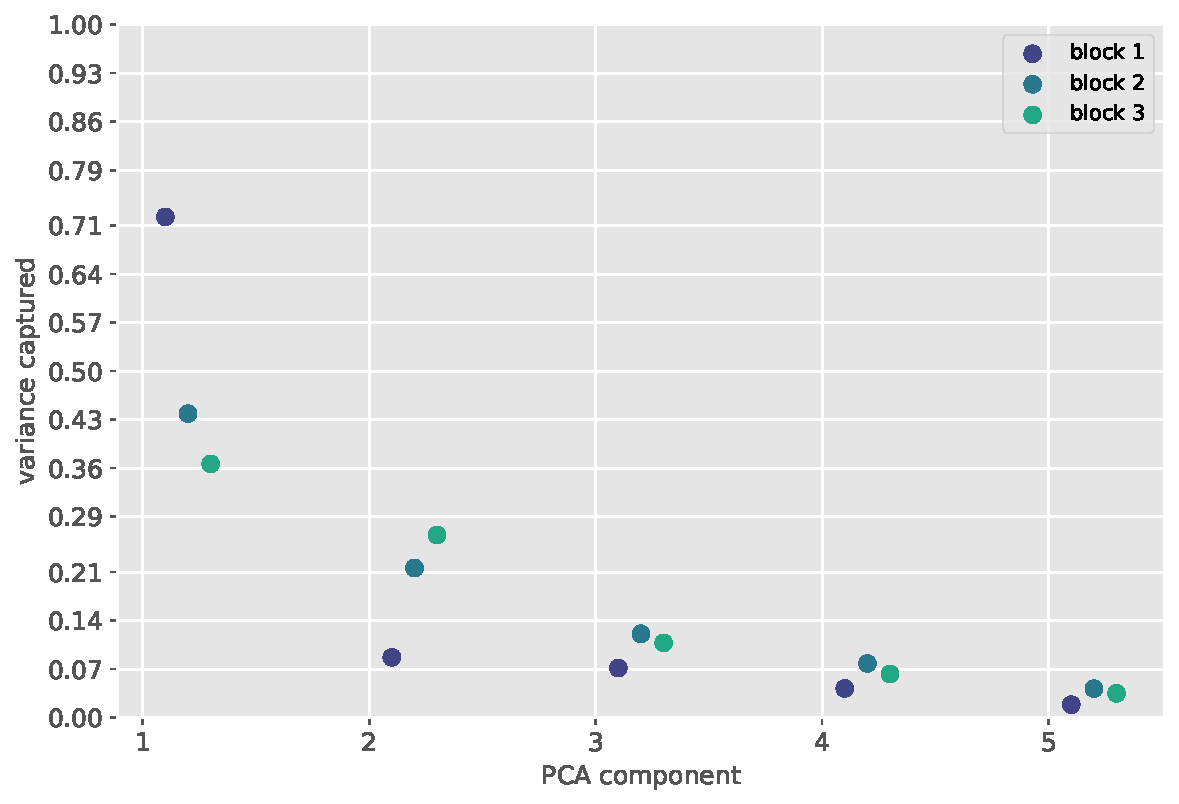
\includegraphics[width=0.7\textwidth,height=\textheight]{images/data_analysis/center_hold/PCA_concat_variance.pdf}
\caption{Fraction of variance captured by PCA computed on concatenated
EMG time series concatenated over trials. Over blocks, we see variance
shifting from the top component to other components. We hypothesize that
across learning we would see the development of bespoke modes used in
combination to reach individual targets. This would predict an increase
in the complexity of the EMG time series over learning. Here we see
suggestions of this prediction.}\label{fig:PCA_concat_variance}
\end{figure}

% <!-- I would be most interested to hear how u are thinking of approaching the analysis. I.e. u have a bunch of channels, movements, tasks what is the workflow to get from that raw data into something manageable/useful. -->
% <!-- The long term goal of the research direction suggested here is to develop tasks which ask subjects to produce a variety of movements in response to a variety of goals and perturbations. This will allow us to study the computations that humans use in everyday tasks to solve the motor problems they face. This stands in contrast to many repetitions of the same movements. However, we wish to validate our experimental setup on classical tasks as a stepping stone to tasks with greater variety. -->
% <!-- "we know how to design and interpret experiments that involve many repetitions of the same movement however there is limited role for online optimization in that context. instead we need experiments where subjects are required to come up with new movements all the time. how can we get experimenters to do such experiments? show cool movies of robots doing cool things,and hopefully get the experimenters excited." (todorov online optimization slides) -->
% <!-- Electrode data from a single trial of a single session is held in a data matrix $X$ (n_electrodes, n_samples), and we wish to find a latent weight matrix $W$ (n_electrodes, n_components) which reconstructs $X$ by projecting latent trajectories $H$ (n_components, n_samples) into electrode space:

% $$
% X = W\cdot{H}
% $$

% $H$ is the activity of the latent processes, and $W$ is there mixing matrix. The columns of $W$ are the principal vectors spanning the latent subspace in electrode space. If we have new samples, we can project these new points onto this subspace:

% $$
% h_{new} = W^T\cdot{w_{new}}
% $$

% To justify this decomposition, we have to make some assumptions about the nature of the EMG signal, namely that the signal is linear instantaneous (each EMG sample can be instantly mapped to control space). The other assumption is that the basis $W$ should be orthonormal, that the columns of $W$ are orthogonal with unity norm. This ensures that the left inverse $W^{-1}$ is equal to the transpose $W^T$ such that:

% \begin{align*}
% X &= W\cdot{H} \\
% W^{-1}\cdot{X} &= {H} \\
% W^{T}\cdot{X} &= {H}
% \end{align*}

% See *Muceli 2014* for use of the Moore-Penrose pseudoinverse in place of the transpose when the columns of $W$ do not form an orthonormal basis. This would be the case for NMF. Is there a factorization that produces nonnegative, orthogonal coordinates? Or is the pseudoinverse okay? I will need to test this.

% Stated in an information theoretic way, we want to minimize the reconstruction loss $\mathcal{L}$ for our derived encoder-decoder pair ($E$,$D$). We're decoding high dimensional activity into its latent dimensions, and encoding back into the high dimensional space. :

% $$
% \min_{E,D}{\mathcal{L}\left[X - EDX\right]}
% $$

% This way, forget about orthonormality and solve for an encoder and decoder directly. That is, $E\neq{D}$ is perfectly acceptable.

% Each row of $D$ might be called a **spatial filter**, a linear combination of electrode activities into a surrogate, hopefully more intuitive space.

% In general to find such a basis we must :

% --> 
% <!-- 1. System Identification -- learning a transition function $p(y_t|x_t, u_t)$
%     - How do you learn the unknown observation model from data?

% 1. Policy Optimization
%     - Once dynamics are learned (or at least stable?), how do we form a policy that is generalizable to new tasks under these dynamics?
%     - This is the control problem.

% It's safe to assume that these processes are happening in parallel. Because we have complete and arbitrary control over the observation mapping, we can ask the subject to interact through a  dynamic that is intuitive (informative prior) or unintuitive (uninformative or inhibitive prior). Each scenario, we hypothesize, will elicit different strategies for learning and control.

% -->